%%%%%%%%%%%%%%%%%%%%%%%%%%%%%%%%%%%%%%%%%
% Short Sectioned Assignment
% LaTeX Template
% Version 1.0 (5/5/12)
%
% This template has been downloaded from:
% http://www.LaTeXTemplates.com
%
% Original author:
% Frits Wenneker (http://www.howtotex.com)
%
% License:
% CC BY-NC-SA 3.0 (http://creativecommons.org/licenses/by-nc-sa/3.0/)
%
%%%%%%%%%%%%%%%%%%%%%%%%%%%%%%%%%%%%%%%%%

%----------------------------------------------------------------------------------------
%	PACKAGES AND OTHER DOCUMENT CONFIGURATIONS
%----------------------------------------------------------------------------------------

\documentclass[paper=a4, fontsize=11pt]{scrartcl} % A4 paper and 11pt font size

\usepackage[T1]{fontenc} % Use 8-bit encoding that has 256 glyphs
\usepackage{fourier} % Use the Adobe Utopia font for the document - comment this line to return to the LaTeX default
\usepackage[english]{babel} % English language/hyphenation
\usepackage{amsmath,amsfonts,amsthm} % Math packages
\usepackage{enumerate}
\usepackage{lipsum} % Used for inserting dummy 'Lorem ipsum' text into the template

\usepackage{sectsty} % Allows customizing section commands
\allsectionsfont{\centering \normalfont\scshape} % Make all sections centered, the default font and small caps
\sectionfont{\raggedright}
\usepackage[english]{babel}
\usepackage{mathtools}
\usepackage{graphicx}
\graphicspath{ {img/} }
\usepackage{pbox}


\usepackage{fancyhdr} % Custom headers and footers
\pagestyle{fancyplain} % Makes all pages in the document conform to the custom headers and footers
\fancyhead{} % No page header - if you want one, create it in the same way as the footers below
\fancyfoot[L]{} % Empty left footer
\fancyfoot[C]{} % Empty center footer
\fancyfoot[R]{\thepage} % Page numbering for right footer
\renewcommand{\headrulewidth}{0pt} % Remove header underlines
\renewcommand{\footrulewidth}{0pt} % Remove footer underlines
\setlength{\headheight}{13.6pt} % Customize the height of the header

\numberwithin{equation}{section} % Number equations within sections (i.e. 1.1, 1.2, 2.1, 2.2 instead of 1, 2, 3, 4)
\numberwithin{figure}{section} % Number figures within sections (i.e. 1.1, 1.2, 2.1, 2.2 instead of 1, 2, 3, 4)
\numberwithin{table}{section} % Number tables within sections (i.e. 1.1, 1.2, 2.1, 2.2 instead of 1, 2, 3, 4)

\setlength\parindent{0pt} % Removes all indentation from paragraphs - comment this line for an assignment with lots of text

%----------------------------------------------------------------------------------------
%	TITLE SECTION
%----------------------------------------------------------------------------------------

\newcommand{\horrule}[1]{\rule{\linewidth}{#1}} % Create horizontal rule command with 1 argument of height

\title{	
\normalfont \normalsize 
\textsc{National Taiwan University, \\ Graduate Institute of Biomedical Engineering and Bioinformatics} \\ [25pt] % Your university, school and/or department name(s)
\horrule{0.5pt} \\[0.4cm] % Thin top horizontal rule
\huge Mathematical Modeling of System Biology \\ Homework 1 \\ % The assignment title
\horrule{2pt} \\[0.5cm] % Thick bottom horizontal rule
}

\author{Yi Hsiao} % Your name

\date{\normalsize\today} % Today's date or a custom date
\begin{document}

\maketitle % Print the title

%----------------------------------------------------------------------------------------
%	PROBLEM 1
%----------------------------------------------------------------------------------------
\newpage
\section{}
Complete the following table. Assume mass action kinetics for all reaction mechanisms.

\begin{center}
    \begin{tabular}{| l | l | l | l |}
    \hline
    &Interaction graph&Rate equation scheme&ODE\\ \hline
	a) & $\xrightarrow{} A\xrightarrow{}$ & \raisebox{-\totalheight}{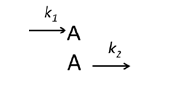
\includegraphics{1a}} & $\frac{d\left[A\right]}{dt}=k_{1}-k_{2}\left[A \right]$\\ \hline
    b) & \raisebox{-\totalheight}{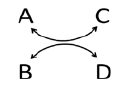
\includegraphics{1b}} & $A+B\xrightleftharpoons[k_{-1}]{k_{1}}C+D$ & \parbox{5cm}{$\frac{d\left[A\right]}{dt}=-k_{1}\left[A \right]\left[B \right]+k_{-1}\left[C \right]\left[D \right]$,\\ $\frac{d\left[B\right]}{dt}=-k_{1}\left[A \right]\left[B \right]+k_{-1}\left[C \right]\left[D \right]$, \\ $\frac{d\left[C\right]}{dt}=k_{1}\left[A \right]\left[B \right]-k_{-1}\left[C \right]\left[D \right]$, \\ $\frac{d\left[D\right]}{dt}=k_{1}\left[A \right]\left[B \right]-k_{-1}\left[C \right]\left[D \right]$} \\ \hline
    c) & \raisebox{-\totalheight}{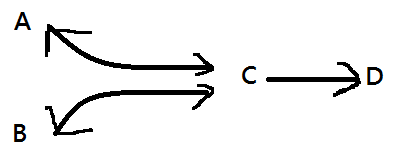
\includegraphics[scale=0.35]{1c-1}} & \parbox{5cm}{$A+B\xrightleftharpoons[k_{-1}]{k_{1}}C\xrightarrow{k_{2}} D$} & \raisebox{-\totalheight}{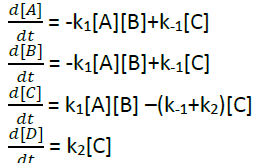
\includegraphics[scale=0.7]{1c}}  \\\hline
    d) & \raisebox{-\totalheight}{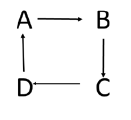
\includegraphics{1d}} & \parbox{5cm}{$A\xrightarrow{k_{1}}B$ \\ $B\xrightarrow{k_{2}}C$\\ $C\xrightarrow{k_{3}}D$ \\ $D\xrightarrow{k_{4}}A$ } & \parbox{5cm}{$\frac{d\left[A\right]}{dt}=-k_{1}\left[A \right]+k_{4}\left[D \right]$ \\ $\frac{d\left[B\right]}{dt}=-k_{2}\left[B \right]+k_{1}\left[A \right]$ \\ $\frac{d\left[C\right]}{dt}=-k_{3}\left[C \right]+k_{2}\left[B \right]$ \\ $\frac{d\left[D\right]}{dt}=-k_{4}\left[D \right]+k_{3}\left[C \right]$}  \\\hline
    e) & \raisebox{-\totalheight}{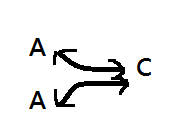
\includegraphics{1e-1}} & \raisebox{-\totalheight}{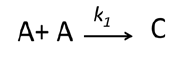
\includegraphics{1e}} & \parbox{5cm}{$\frac{d\left[A\right]}{dt}=-2k_{1}\left[A \right]^{2}$, \\ $\frac{d\left[C\right]}{dt}=k_{1}\left[A \right]^{2}$}\\\hline
    \end{tabular}
\end{center}

\subsection{Problem Set 2.4.7 Network modelling.}
	\begin{enumerate}[a)]
		\item Consider the closed reaction network in Figure 2.16 with reaction rates $v_{i}$ as indicated. Suppose that the reaction rates are given by mass action as $v_{1}= k_{1}\left[ A \right]\left[ B \right]$, $v_{2} = k_{2}\left[ D \right]$ and $v_{3} = k_{3}\left[ C \right]$.
		\begin{enumerate}[i)]
			\item Construct a differential equation model for the network. Use moiety conservations to reduce your model to three differential equations and three algebraic equations.

			Initially, we can construct a set of differential equations of every species.
			\begin{align*}
				\frac{d\left[ A \right]}{dt}&=-v_{1},&\frac{d\left[ B \right]}{dt}&=-v_{1}+v_{2},&
				\frac{d\left[ C \right]}{dt}&=v_{1}-v_{3},&\\
				\frac{d\left[ D \right]}{dt}&=v_{1}-v_{2},&\frac{d\left[ E \right]}{dt}&=v_{3},&
				\frac{d\left[ F \right]}{dt}&=v_{3}
			\end{align*}
			Then, we can further combine many differential equations to make this set of equations smaller, because there are only three independent variables. Actually, we only need three linearly independent equations. That is, the three differential equations can be derived by moiety conservations: \\
			\begin{align*}
				\frac{d\left[ A \right]}{dt}+\frac{d\left[ C \right]}{dt}+\frac{d\left[ E \right]}{dt}&=0,&
				\frac{d\left[ A \right]}{dt}+\frac{d\left[ C \right]}{dt}+\frac{d\left[ F \right]}{dt}&=0,&
				\frac{d\left[ B \right]}{dt}+\frac{d\left[ D \right]}{dt}&=0&
			\end{align*}
			where the three algebraic equations are
			\begin{align*}
				v_{1}&=k_{1}\left[ A \right]\left[ B \right],&v_{2}&=k_{2}\left[ D \right],&v_{3}&=k_{3}\left[ C \right]
			\end{align*}

			\item Solve for the steady-state concentrations as functions of the rate constants and the initial concentrations. (Note, because the system is closed, some of the steady-state concentrations are zero.)

			Let us denote by $a_{0}$ and $b_{0}$ the initial concentration. According to the three differential equations derived from i), we can further derive :\\
			$\frac{d\left[ A \right]}{dt}+\frac{d\left[ C \right]}{dt}+\frac{d\left[ E \right]}{dt}=0\Rightarrow
			\frac{d(\left[ A \right]+ \left[C \left]+\right[ E \right])}{dt}=0\Rightarrow
			\left[ A \right]+ \left[C \left]+\right[ E \right]=constant=a_{0}\\
			\frac{d\left[ A \right]}{dt}+\frac{d\left[ C \right]}{dt}+\frac{d\left[ F \right]}{dt}=0\Rightarrow
			\frac{d(\left[ A \right]+ \left[C \left]+\right[ F \right])}{dt}=0\Rightarrow
			\left[ A \right]+ \left[C \left]+\right[ F \right]=constant=a_{0}\\
			\frac{d\left[ B \right]}{dt}+\frac{d\left[ D \right]}{dt}=0\Rightarrow
			\frac{d(\left[ B \right]+\left[ D \right])}{dt}=0\Rightarrow
			\left[ B \right]+\left[ D \right]=constant=b_{0}$\\

			These equations should be hold all the time. Let us denote by $[I]_{ss}$ the steady state concentration of the species I. Then, we can further derive that:\\
			$\left[ A \right]_{ss}+ \left[C \left]_{ss}+\right[ E \right]_{ss}=\left[C \left]_{ss}+\right[ E \right]_{ss}=a_{0}\\
			\left[ A \right]_{ss}+ \left[C \left]_{ss}+\right[ F \right]_{ss}=\left[C \left]_{ss}+\right[ F \right]_{ss}=a_{0}$\\
			
			It's because that there is no supply for A, A will be zero eventually. Additionally,
			$v_{1}=k_{1}\left[ A \right]_{ss}\left[ B \right]_{ss}=0$ at steady state will induce that there is no supply for C and D either, so we can conclude that\\
			$\left[ C \right]_{ss}=0\Rightarrow\left[ E \right]_{ss}=a_{0}, \left[ F \right]_{ss}=a_{0}\\
			\left[ D \right]_{ss}=0\Rightarrow\left[ B \right]_{ss}=b_{0}$
			
			by further substituting the concentration at steady state back to the constant condition derived above. In summary, $\left[ A \right]_{ss}=0, \left[ B \right]_{ss}=b_{0}, \left[ C \right]_{ss}=0, \left[ D \right]_{ss}=0, \left[ E \right]_{ss}=a_{0}, \left[ F \right]_{ss}=a_{0}$

			\item Verify your result in part (ii) by running a simulation of the system from initial conditions (in mM) of ($\left[ A\right], \left[B\right], \left[C\right], \left[D\right], \left[E\right], \left[F\right]) = (1, 1, \frac{1}{2} , 0, 0, 0)$. Take rate constants $k_{1} = 3$/mM/sec, $k_{2} = 1$/sec, $k_{3} = 4$/sec.

		\end{enumerate}
		\item Next consider the open system in Figure 2.17 with reaction rates vi as indicated. Suppose that the reaction rates are given by mass action as $v_{0} = k_{0}, v_{1} = k_{1}\left[A\right]\left[B\right], v_{2} = k_{2}\left[D\right], v_{3} = k_{3}\left[C\right], v_{4} = k_{4}\left[E\right]$, and $v_{5} = k_{5}\left[F\right]$.

		\begin{enumerate}[i)]
			\item Construct a differential equation model for the network. Identify any moiety conservations in the network.

			The thoughts here are similar to part (a). Initially, we can construct a set of differential equations of every species.
			\begin{align*}
				\frac{d\left[ A \right]}{dt}&=v_{0}-v_{1},&\frac{d\left[ B \right]}{dt}&=-v_{1}+v_{2},&
				\frac{d\left[ C \right]}{dt}&=v_{1}-v_{3},&\\
				\frac{d\left[ D \right]}{dt}&=v_{1}-v_{2},&\frac{d\left[ E \right]}{dt}&=v_{3}-v_{4},&
				\frac{d\left[ F \right]}{dt}&=v_{3}-v_{5}
			\end{align*}
			Then, we can further combine many differential equations. Then, the three moiety conservations can be derived: 
			\begin{align*}
				\frac{d\left[ A \right]}{dt}+\frac{d\left[ C \right]}{dt}+\frac{d\left[ E \right]}{dt}&=v_{0}-v_{4},&
				\frac{d\left[ A \right]}{dt}+\frac{d\left[ C \right]}{dt}+\frac{d\left[ F \right]}{dt}&=v_{0}-v_{5},&
				\frac{d\left[ B \right]}{dt}+\frac{d\left[ D \right]}{dt}&=0&
			\end{align*}
			where the six algebraic equations are
			\begin{align*}
				v_{0}&=k_{0},&v_{1}&=k_{1}\left[ A \right]\left[ B \right],&v_{2}&=k_{2}\left[ D \right],&v_{3}&=k_{3}\left[ C \right],&v_{4}&=k_{4}\left[E\right],&v_{5}&=k_{5}\left[F\right]&
			\end{align*}

			\item Solve for the steady state as a function of the rate constants and the initial concentrations.

			 We can first derive following mathematical relationships by using the fact that all change rates of species equals to zero at steady state and moiety conservations, that is:\\
			$\frac{d\left[ A \right]}{dt}+\frac{d\left[ C \right]}{dt}+\frac{d\left[ E \right]}{dt}=v_{0}-v_{4}=v_{0}-k_{4}\left[E\right]_{ss}=0\Rightarrow \left[E\right]_{ss}=\frac{v_{0}}{k_{4}}=\frac{k_{0}}{k_{4}}\\
			\frac{d\left[ A \right]}{dt}+\frac{d\left[ C \right]}{dt}+\frac{d\left[ F \right]}{dt}=v_{0}-v_{5}=v_{0}-k_{5}\left[F\right]_{ss}=0\Rightarrow \left[F\right]_{ss}=\frac{v_{0}}{k_{5}}=\frac{k_{0}}{k_{5}}\\
			\frac{d\left[ B \right]}{dt}+\frac{d\left[ D \right]}{dt}=0\Rightarrow \frac{d(\left[ B \right]+\left[ D \right])}{dt}=0\Rightarrow
			\left[ B \right]+\left[ D \right]=constant=b_{0}=\left[ B \right]_{ss}+\left[ D \right]_{ss}$\\
			at steady-state. Also, at steady-state,\\

			$\frac{d\left[ A \right]}{dt}=v_{0}-v_{1}=0\Rightarrow v_{0}=v_{1}\\
			\frac{d\left[ D \right]}{dt}=v_{1}-v_{2}=0\Rightarrow v_{1}=v_{2}\\
			\frac{d\left[ C \right]}{dt}=v_{1}-v_{3}=0\Rightarrow v_{1}=v_{3}\\
			$
			Then, we can combine these two equation with the rate change of D at steady-state:\\
			$v_{0}=v_{2}=k_{2}\left[D\right]_{ss} \Rightarrow \left[D\right]_{ss}=\frac{v_{0}}{k_{2}}=\frac{k_{0}}{k_{2}} \Rightarrow \left[ B\right]_{ss}=b_{0}-\left[D\right]_{ss}=b_{0}-\frac{k_{0}}{k_{2}} \Rightarrow v_{0} = v_{1} = k_{1}\left[ A\right]_{ss}\left[B \right]_{ss}\\\Rightarrow \left[ A\right]_{ss}=\frac{v_{0}}{k_{1}\left[ B\right]_{ss}}=\frac{k_{0}}{k_{1}(b_{0}-\frac{k_{0}}{k_{2}})}\\
			v_{0}=v_{3}=k_{3}\left[C\right]_{ss}\Rightarrow \left[C\right]_{ss}=\frac{v_{0}}{k_{3}}=\frac{k_{0}}{k_{3}}$

			\item Verify your result in (ii) by running a simulation of the system from initial conditions (in mM) of ($\left[A\right], \left[B\right], \left[C\right], \left[D\right], \left[E\right], \left[F\right]) = (1, 1, \frac{1}{2} , 0, 0, 0)$. Take rate constants $k_{0} = 0.5 mM/sec, k_{1} = 3/mM/sec, k_{2} = 1/sec, k_{3} = 4/sec, k_{4} = 1/sec, k_{5} = 5/sec$.
			\item Given the initial conditions and rate constants in part (iii), why would there be no steady state if we take $k_{0} = 5 mM/sec$?
		\end{enumerate}

	\end{enumerate}

\subsection{Problem Set 2.4.8 Rapid equilibrium approximation.}
	Consider the closed system:\\
	\\
	with mass action rate constants as shown. Suppose the rate constants are (in min\textsuperscript{-1}) $k_{1} = 0.05, k_{2} = 0.7, k_{-1} = 0.005, and k_{-2} = 0.4$.
	\begin{enumerate}[a)]
		\item Construct a differential equation model of the system. Simulate your model with initial conditions (in mM) of A(0) = 1.5, B(0) = 3, C(0) = 2. Plot the transient and steady-state behaviour of the system. You may need to make two plots to capture all of the dynamics (i.e. two different window sizes).

		\item It should be clear from your simulation in part (a) that the system dynamics occur on two different time-scales. This is also apparent in the widely separated rate constants. Use a rapid equilibrium assumption to reduce your description of the system to two differential equations (de- scribing one of the original species and one combined species pool) and two algebraic equations (describing the contents of the combined pool).

		\item Run a simulation of your reduced model in part (b) to compare with the simulation in part (a). Verify that the simulation of the reduced system is in good agreement with the original, except for a short initial transient. (Note, you will have to select initial conditions for the reduced system so that the initial total concentration is in agreement with part (a), and the rapid equilibrium condition is satisfied at time t = 0.)
	\end{enumerate}
\subsection{Problem Set 2.4.9 Quasi-steady-state approximation.}
	Consider the reaction network:\\
	\\
	Suppose the mass action rate constants are (in min\textsuperscript{-1}) $k_{0}=1, k_{1} = 11, k_{-1} = 8,$ and $k_{2} = 0.2$.
	\begin{enumerate}
		\item Construct a differential equation model of the system. Simulate your model with initial conditions A(0) = 6 mM, B(0) = 0 mM. Plot the transient and steady-state behaviour of the system. You may need to make two plots to capture all of the dynamics (i.e. two different window sizes).


		\item It should be clear from your simulation in part (a) that the system dynamics occur on two different time-scales. This is also apparent in the widely separated rate constants. Use a quasi-steady-state assumption to reduce your description of the system by replacing a differential equation with an algebraic equation.
		\item Run a simulation of your reduced model in part (b) to compare with the simulation in part (a). Verify that the simulation of the reduced system is a good approximation to the original at steady state, but not over the initial transient. (Note, you will have to select initial conditions for the reduced system so that the total concentration is in agreement with part (a), and the quasi-steady state condition is satisfied at time t = 0, as in Exercise 2.2.4.)
	\end{enumerate}
\end{document}